% 
% NTHU Template
% 2014 Yao Wei
%
% This file is licensed under CC0.
% https://creativecommons.org/publicdomain/zero/1.0/
%

\documentclass[12pt]{article}

% Lint
\RequirePackage[l2tabu, orthodox]{nag}

% Fonts
\usepackage{mathptmx}
\usepackage[T1]{fontenc}
\usepackage{CJKutf8}

% Layout
\usepackage[a4paper, top=2.54cm, bottom=2.54cm, left=3.17cm, right=2.54cm]{geometry}
\usepackage{abstract}

% Paragraph
\usepackage{indentfirst}
\usepackage{setspace}

\usepackage{tabularx}

% Watermarks
\usepackage{wallpaper}
\CenterWallPaper{.18}{./assets/nthu_watermark.eps}
\setlength{\wpXoffset}{0.315cm}

% Citations

\usepackage[backend=bibtex,sorting=none,maxcitenames=2,maxbibnames=3,hyperref=true,block=none]{biblatex}
\bibliography{thesis}
\renewbibmacro{in:}{}

% Figures
\usepackage{float}
\usepackage{subcaption}
\usepackage{rotating}

\begin{document}
\begin{CJK}{UTF8}{bkai}

\begin{titlepage}
\begin{center}
\Huge 國~立~清~華~大~學 \\ [1.5ex]
\Huge \underline{碩~士~論~文} \\
%\Large (初稿)\\
\vspace*{10ex}
\huge 適用於異質系統架構的數位訊號處理器設計 \\
\vspace*{1ex}
\huge Design of Digital Signal Processor for Heterogeneous System Architecture  \\

\null
\vfill

\Large
\begin{tabular}{r@{\centering} @{}l}
    系\ 所\ 別:~&電機工程學系碩士班\ \ \ 組別:系統組	\\ [1.5ex]
    學號姓名:~&103061568~李齊明~(Chi-Ming~Lee)      \\ [1.5ex]
    指導教授:~&許雅三~博士~(Prof.~Yarsun~Hsu)       \\
	
\end{tabular}

\vspace*{2ex}
\Large 中華民國 105 年 6 月
\end{center}
\end{titlepage}

\doublespacing
\pagenumbering{roman}
\setcounter{page}{3}
\addcontentsline{toc}{section}{Abstract}

\renewcommand{\abstractnamefont}{\normalfont\bfseries}
\renewcommand{\abstracttextfont}{\normalfont}
\setlength{\absleftindent}{0pt}
\setlength{\absrightindent}{0pt}

\begin{abstract}  % Abstract
	Will be done last.
\end{abstract}
\clearpage
\addcontentsline{toc}{section}{Acknowledgements}

\begin{center}
\textbf{Acknowledgements}
\end{center}
Acknowledgements Page
\clearpage

\singlespacing

\tableofcontents  % Table of contents
\clearpage
\addcontentsline{toc}{section}{List of Figures}
\listoffigures  % List of figures
\clearpage
\addcontentsline{toc}{section}{List of Tables}
\listoftables  % List of tables
\clearpage

\doublespacing
%\setlength{\parskip}{12pt}

\pagenumbering{arabic}

\section{Introduction}

    \subsection{Motivation}
        As wireless communication standard evolves, the demand for digital signal processing platform that supplies computation with high-performance, high-flexibility and low-energy consumption is gaining momentum in the mobile industry. 
        Take an example of LTE-advance, which is considered to be the next mainstream mobile wireless technology, it provides 10 times higher transmission throughput than that of LTE \cite{lte}. 
        In order to achieve this enhancement, strategies such as scaling up MIMO system and permitting carrier aggregation \cite{carrier} that require more sophisticated arithmetics are adopted in LTE-advance.
        Moreover, these algorithms used in LTE-advance demodulation will still change frequently with the protocol specification.
        Consequently, both energy efficiency and flexibility become crucial considerations in the filed of digital signal processor implementation. 
        However, VLIW and ASIP, which have been popular choices of state-of-the-art digital signal processor (DSP) micro-architecture, serve as two extremes cases for hardware designers who would like to trade-off between flexibility and energy efficiency. 
        VLIW gains good flexibility by allocating each functional unit dedicated control signals and ports on register file that result in significant power dissipation, so it could work orthogonally with each other; 
        On the contrary, ASIP benefits from optimized data-path for the specific ISA or algorithm by sacrificing its flexibility so good energy efficiency is achieved. 
        Consequently, improving energy efficiency while keeping hardware flexibility for DSP on mobile devices becomes a challenge.	\\

        On the other hand, heterogeneous computing, which refers to systems equipped with multiple types of processors, has opened a new era for digital signal processing. 
        Such an integration of different processors gains performance improvement by taking advantage of particular processing activities to handle certain types of tasks.
        Nowadays, a digital signal processing platform typically contains a CPU that handles control intensive tasks and a DSP that perform computation intensive ones.
        Nevertheless, in such heterogeneous DSP platforms, there is still a drawback owing to the communication latency between processors. 
        Frequent data transfer and task dispatching control between DSP and CPU lead to a  bottleneck of performance. 
        As a result, HSA foundation, found by AMD, ARM, MediaTek, etc, propose a new standard for heterogeneous computing, HSA system specification \cite{systemspec}, to address the problem. 
        The standard creates concepts of unified memory space and architectural queuing language that alleviate burdens on data transfer and task dispatching, becoming the potential mainstream of computer architecture in the future \cite{mainstream}.

    \subsection{Goal and Contribution}
        To improve performance and energy efficiency as well as maintain flexibility for digital signal processing platforms, we propose a hybrid VLIW-TTA DSP, and present a framework which integrates the processor with HSA platforms which are able to reduce communication overhead between CPU and DSP. Prominent micro-architectural features of the proposed DSP include:
        \begin{itemize}
            \item The VLIW-style data-path activates multiple functional units in a cycle. High operations per cycle (OPC) can be achieved with proper scheduling.
            \item TTA-style transport-triggered scheduling aggressively forwards data from accumulators to functional units. Unnecessary data write-back can be avoided so energy dissipation in register file is consequently reduced.
            \item Banked organization of register file eliminates redundant connections from ports to registers. Compared with the conventional centralized organization, both power consumption and circuit area are saved.
            \item Register file access is regularized to a queue/stack operation (i.e. push or pop) instead of conventional random access, which requires more bits to specify a register address. Density of VLIW-style code can be improved.
            \item The data-path is suitable for clustering and it can be scaled up to SIMD or vector-processing architectures.
        \end{itemize}
        In addition, to evaluate the proposed processor with existing architectures, we selected several classical DSP kernels \cite{dspstone} \cite{bdti} as the benchmark and use the UMC 65nm CMOS technology to implement the hardware.

        The main contribution of this work is achieve at two levels: micro-architecture and HSA level. 
        On the micro-architecture side, with equal resources of functional unit and register file, the proposed hybrid processor outperformed by 30\% in MOPS\/mW and improve 50\% in code density while remaining competitive computational throughput, compared with the conventional VLIW architecture.
        On the HSA side, we present a completed code generation flow for the proposed DSP which meets the requirements from HSA standard, and illustrate the system framework of HSA platforms that run with the proposed VLIW processor.
 
    \subsection{Organization}
        The remainder of this thesis is organized as follows: In Chapter 2, we briefly review work related to our architecture. In Chapter 3, we introduces background knowledge about this work. In Chapter 4, we look into the details of the proposed design. In Chapter 5, we provide experimental results that demonstrate the capabilities of this architecture. Finally, Chapter 6 present conclusions and future work of the thesis.

\newpage

\section{Related Work}
    In the stream of DSP design, many studies have been conducted on register file (RF) organization as it becomes the dominating factor of cycle time, power consumption and chip area \cite{register}.
    Rixner \textit{et al.} indicated that, for conventional centralized organization, the cost grows significantly with the number of functional units (FUs) \cite{register}, causing a challenge for designing VLIW DSP.
    A straightforward solution is partitioning the centralized RF into several parts, each of which serves specific FUs, such as \cite{cluster}.
    Studies like \cite{synzen} and \cite{dsplite} went even further by discarding the centralized RF and allocating each FU a dedicated one, which is also known as distributed RF organization.
    However, dividing RF leads to more complicated compiler design and overhead of inter-RF data transport.
    In addition, above approaches still suffer from poor code density, which is an inherent problem from the VLIW architecture.
    \\
    Some approaches avoided the aforementioned cost growth by customizing the data-path and limiting the number of ports on RF.
    Ou \textit{et al.} proposed composite FUs for DSP, which cascade FUs with a specific order and demand fewer ports on RF \cite{cascade} \cite{hearaid}.
    Similar techniques are often applied to ASIP design but they usually lack flexibility to target general purposes.
    There are further researches that achieve power reduction on RF by minimizing the number of accesses to it.
    Chen \textit{et al.} proposed a simulated-annealing based scheduling that aggressively forwards data from FU outputs to inputs instead of accessing RF \cite{multistage}.
    \cite{move} presented a processor framework: MOVE, which features the separation of data transport and operation in the data-path. 
    The user can program the bypass network in MOVE, and avoid most of accesses to RF by clever data transport.
    Such an architecture that manipulates data transport usually refers to transport-triggered architecture (TTA).
    The Work from Lama \textit{et al.} \cite{ttagpu} also demonstrated a framework that takes the advantage of TTA in graphic processing unit (GPU), and this idea is a potential alternative for DSP design.
    \\
    On the other hand, one may notices that none of the above implementations adopts HSA \cite{systemspec}, which is a promising standard for embedded DSP platforms.
    So far, most of studies on HSA focus on the integration of CPU and GPU. \cite{hsaemu} presented a full system emulator for HSA platforms that include CPUs and GPUs.
    Beyond emulation, \cite{hsacyc} further illustrated a cycle-accurate HSA simulator that integrates QEMU and GPGPU-sim \cite{gpgpusim}.
    To the best of our knowledge, little or no research has been performed to apply the standard to DSP platforms.

\newpage

\section{Background}

    \subsection{Digital Signal Processors}
        \subsubsection{Application-Specific Instruction Set Processor}
        \subsubsection{Very Long Instruction Word Processor}
        \subsubsection{Transport-Triggered Architecture}

    \subsection{Register Files Organization}
        %\subsubsection{Centralized Register Files}
        %\subsubsection{Banked Register Files}
        %\subsubsection{Clustered Register Files}
        %\subsubsection{Distributed Register Files}
    \subsection{Heterogeneous System Architecture}
        \subsubsection{System Specification}
        \subsubsection{Software Stack}

\section{Design and Implementation}
    \subsection{System Overview}
    \subsection{Micro-architecture Design}
        \begin{figure}[!ht]
            \caption{Micro-architecture of the proposed DSP}
            \centering
            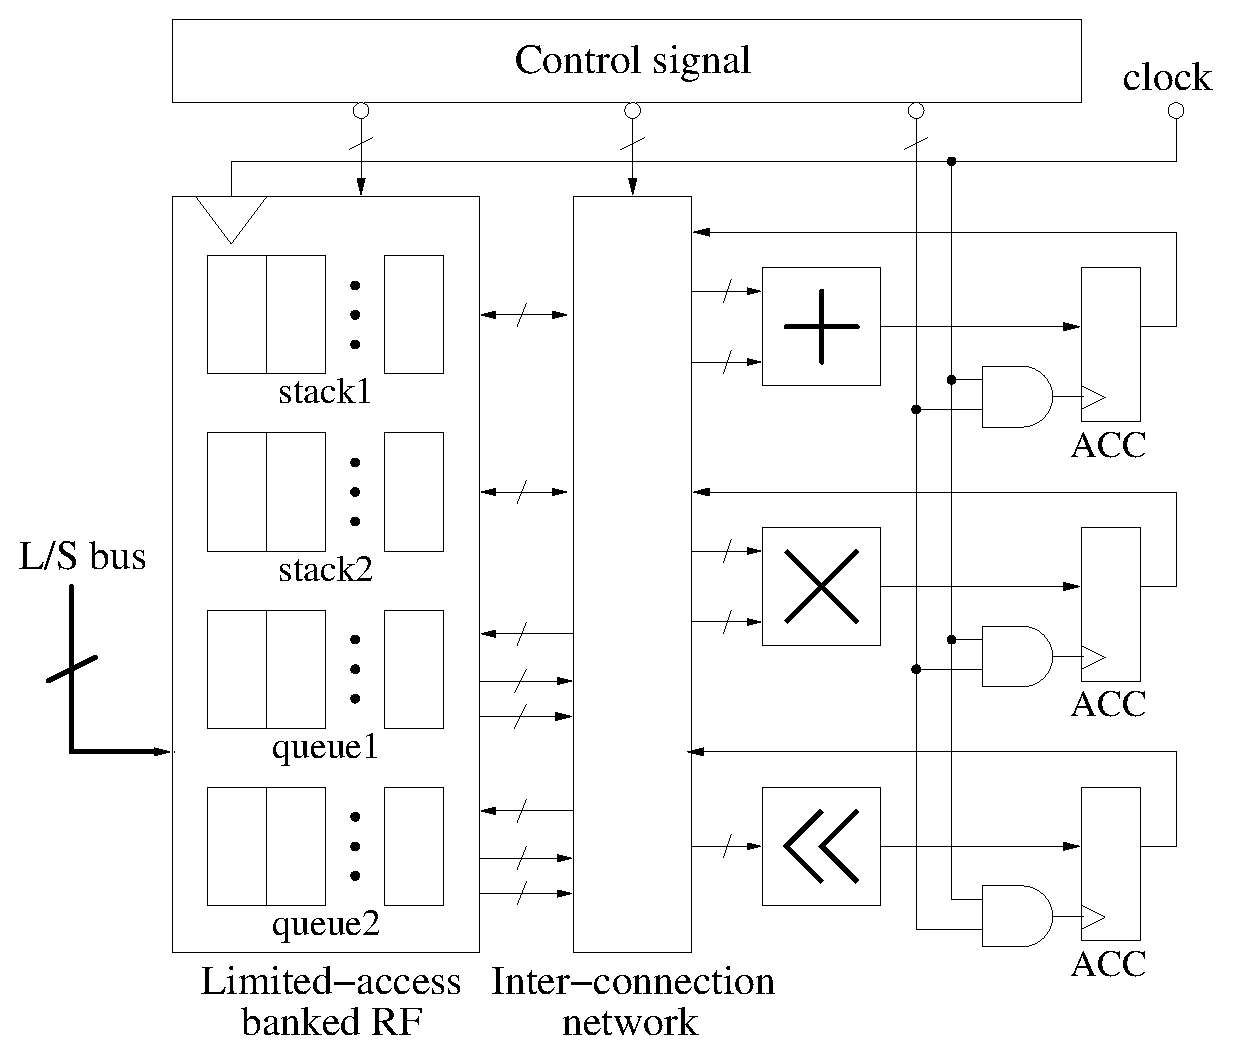
\includegraphics[width=0.8\textwidth]{./figs/micro.eps}
        \end{figure}
    \subsection{Software Design}
        \subsubsection{Compiler Front-end}
        \subsubsection{Finalizer Back-end}

\section{Performance Evaluation}
    \subsection{Operation per Cycle}
    \subsection{Write back per Operation}
    \subsection{MOPS vs Area}
    \subsection{MOPS vs Energy}

\section{Conclusions and Future Work}

\clearpage

\addcontentsline{toc}{section}{References}
\singlespacing
%\setlength{\parskip}{0pt}

\printbibliography

\end{CJK}
\end{document}
